\begin{table}[ht]
\centering
\caption{Completed development pilot accuracy (percent); not a held-out hypothesis test. Each cell retains both worlds and both stochastic repetitions.}
\label{tab:pilot}
\small
\begin{tabular}{lllrrr}
\hline
Task & Organization & Policy & Single & Exact & Paraphrase\\
\hline
schedule & flat & ordinary & 100.0 & 100.0 & 100.0\\
schedule & flat & checklist & 100.0 & 100.0 & 100.0\\
schedule & hierarchical & ordinary & 81.2 & 95.8 & 95.8\\
schedule & hierarchical & checklist & 81.2 & 93.8 & 87.5\\
workflow & flat & ordinary & 87.5 & 83.3 & 87.5\\
workflow & flat & checklist & 87.5 & 87.5 & 91.7\\
workflow & hierarchical & ordinary & 83.3 & 85.4 & 87.5\\
workflow & hierarchical & checklist & 79.2 & 81.2 & 83.3\\
\hline
\end{tabular}
\end{table}
\begin{figure}[ht]
\centering
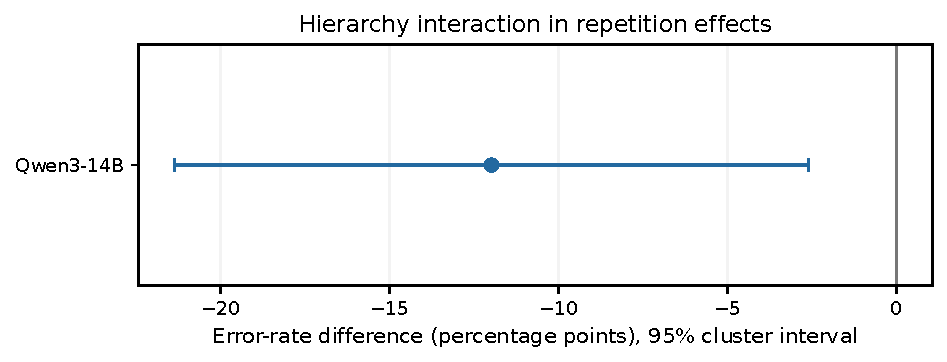
\includegraphics[width=\textwidth]{../results/pilot-v7/figures/hierarchy.pdf}
\caption{Development-only primary scheduling: hierarchy. Intervals, where shown, resample base-instance clusters.}
\label{fig:pilot-hierarchy}
\end{figure}
\begin{figure}[ht]
\centering
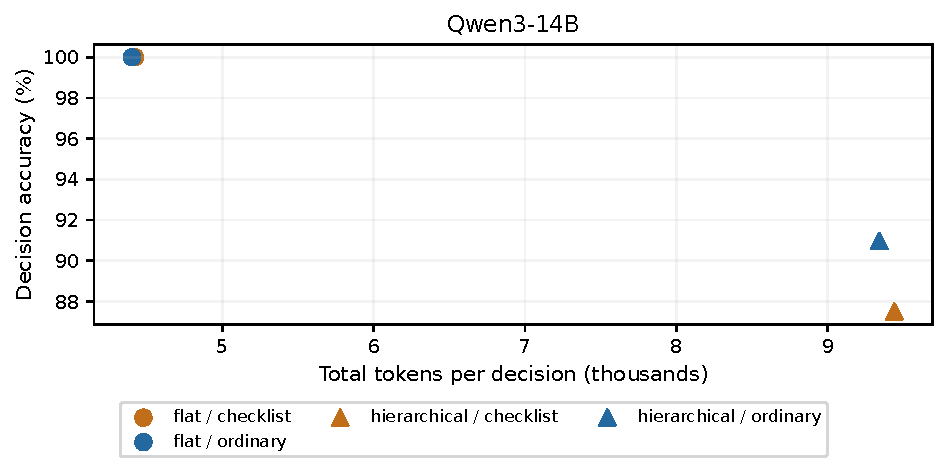
\includegraphics[width=\textwidth]{../results/pilot-v7/figures/resource.pdf}
\caption{Development-only primary scheduling: resource. Intervals, where shown, resample base-instance clusters.}
\label{fig:pilot-resource}
\end{figure}
